
\chapter{کارهای پیشین}

در این فصل، به مرور کارهای پیشین و روش‌های مرتبط ترمیم تصویر پرداخته می‌شود. هدف از این مرور، شناسایی نقاط قوت و ضعف روش‌های موجود، بررسی پیشرفت‌های اخیر در حوزه مرتبط، بررسی مجموعه‌داده های ترمیم تصویر و ارائه یک دیدگاه جامع از متدولوژی های مرسوم ترمیم است.

ابتدا به بررسی تاریخچه و پیشرفت روش‌های مرتبط با ترمیم تصاویر پرداخته خواهد شد و دسته‌بندی‌های مختلف این روش‌ها، به همراه مزایا و معایب آن‌ها مورد بحث قرار خواهد گرفت. سپس، مجموعه داده‌های مورد استفاده در این حوزه معرفی شده و معیارهای مورد نظر برای ارزیابی این روش‌ها توضیح داده می‌شوند. در نهایت، الگوریتم‌های کلاسیک و روش‌های مبتنی بر یادگیری عمیق که تاکنون برای ترمیم تصاویر پیشنهاد شده‌اند، بررسی خواهند شد. \textbf{این تحلیل به عنوان مبنایی برای توجیه ضرورت استفاده از معماری \lr{Transformers} در تحقیق حاضر خواهد بود.}



\section{روش های الگوریتمی}

مسئله ترمیم تصویر به قبل‌تر از ظهور روش‌های مبتنی بر یادگیری عمیق بازمی‌گردد. در ابتدا این مسئله به کمک روش‌های الگوریتمی کلاسیک مورد بررسی قرار گرفت. یکی از اولین روش‌های مطرح‌شده در حوزه ترمیم تصاویر، رویکرد مبتنی بر انتشار بود که توسط Bertalmio و همکارانش در سال ۲۰۰۰ معرفی شد \cite{bertalmioImageInpainting2000}. این روش از معادلات دیفرانسیل جزئی \lr{(PDE)} برای گسترش اطلاعات موجود در لبه‌های تصویر به نواحی آسیب‌دیده استفاده می‌کند. ایده اصلی این روش، شبیه‌سازی فرآیند طبیعی انتشار اطلاعات در تصویر است تا ساختارهای محلی به صورت پیوسته بازسازی شوند. با وجود اینکه این روش برای ترمیم نواحی کوچک و حفظ ساختار لبه‌ها عملکرد خوبی دارد، در بازسازی نواحی بزرگ‌تر یا بافت‌های پیچیده به دلیل محدودیت درک محتوای کلی تصویر ناکارآمد است.

در ادامه رویکردهای مبتنی بر انتشار، روش ترمیم تصویر با تغییرات کل \lr{(Total Variation Inpainting)} که توسط Chan و Shen در سال ۲۰۰۱ معرفی شد \cite{chanNontextureInpaintingCurvatureDriven2001}، گامی دیگر در پیشرفت این حوزه بود. این روش بر مبنای به حداقل رساندن یک تابع انرژی طراحی شده است که هدف آن حفظ ساختار لبه‌ها و جلوگیری از ایجاد تاری در نواحی بازسازی‌شده است. مدل تغییرات کل از معادلات دیفرانسیل جزئی برای انتقال اطلاعات لبه‌ها به نواحی آسیب‌دیده استفاده می‌کند و توانایی بالایی در بازسازی ساختارهای ساده دارد. با این حال، مانند روش Bertalmio و همکاران، این رویکرد نیز در بازسازی بافت‌های پیچیده یا نواحی بزرگ با محدودیت‌هایی مواجه است.


دسته دیگری از روش‌های کلاسیک، روش‌های مبتنی بر وصله \lr{(Patch-Based Methods)} بودند که از آماره‌های غیرمحلی برای بازسازی تصویر استفاده می‌کردند. در این روش‌ها، نواحی سالم تصویر به عنوان بانک وصله‌ها در نظر گرفته می‌شدند و بهترین تطابق برای پر کردن نواحی آسیب‌دیده از میان این وصله‌ها انتخاب می‌شد.

به‌عنوان مثال در یکی از برجسته ترین روش های غیرمبتنی بر یادگیری، بارنز و همکاران در \cite{barnesPatchMatchRandomizedCorrespondence2009} با معرفی PatchMatch ابزارهای تعاملی ویرایش تصویر را با استفاده از یک الگوریتم تصادفی جدید ارائه داده‌اند که امکان یافتن بسیار سریع تطابق‌های تقریبی نزدیک‌ترین همسایه بین قطعات تصویر را فراهم می‌کند. الگوریتم ارائه‌شده توسط آن‌ها بهبودهای قابل‌توجهی در عملکرد نسبت به روش‌های پیشین (۲۰ تا ۱۰۰ برابر سریع‌تر) ارائه می‌دهد و استفاده از آن را در ابزارهای تعاملی ممکن می‌سازد. بینش‌های کلیدی این الگوریتم شامل یافتن برخی تطابق‌های مناسب از طریق نمونه‌گیری تصادفی و استفاده از هم‌بستگی طبیعی در تصاویر برای انتشار سریع این تطابق‌ها به نواحی مجاور است.

با وجود این که این رویکردها توانستند نتایج بهتری در بازسازی جزئیات ارائه دهند، اما به دلیل تکیه بر ویژگی‌های محلی و وابستگی به مشابهت بافتی، در مواجهه با تصاویر پیچیده و متنوع محدودیت‌های زیادی داشتند.


\section{روش‌های مبتنی بر یادگیری عمیق}

با ظهور یادگیری عمیق و توانایی آن در استخراج ویژگی‌های پیچیده از داده‌های تصویری، پژوهش‌ها در زمینه ترمیم تصاویر به سمت استفاده از مدل‌های مبتنی بر شبکه‌های عصبی سوق یافت. این روش‌ها با استفاده از مجموعه داده‌های بزرگ و متنوع، قادر به یادگیری الگوهای پیچیده و بازسازی دقیق‌تر نواحی آسیب‌دیده شدند. برخلاف روش‌های الگوریتمی که عمدتاً بر اصول ریاضی و آماری استوار بودند، روش‌های مبتنی بر یادگیری امکان درک مفاهیم سطح بالا و روابط جهانی در تصویر را فراهم کردند و موفق شدند ترمیم هایی با  ماسک های بزرگ‌تر انجام دهند، چرا که این امر گاها نیازمند ساخت ساختار های کاملا جدید در تصویر (مانند ساختار چهره، طبیعت و ...) بود.



در مقایسه با روش‌های سنتی، روش‌های مبتنی بر یادگیری در ترمیم تصاویر موفقیت چشمگیری کسب کرده‌اند، به‌ویژه زمانی که صحبت از تولید محتوای جدید و همخوان با زمینه برای نواحی بزرگ حذف‌شده باشد.

Pathak
و همکاران در \cite{pathakContextEncodersFeature2016}
یک الگوریتم یادگیری ویژگی‌های بصری بدون نظارت \LTRfootnote{Unsupervised} ارائه داده‌اند که بر اساس پیش‌بینی پیکسل مبتنی بر زمینه هدایت می‌شود. به‌طور مشابه با خودرمزگذارها
\LTRfootnote{Autoencoders}
، آن‌ها \lr{Context Encoders} را پیشنهاد کرده‌اند – یک شبکه عصبی کانولوشنی که برای تولید محتوای یک ناحیه دلخواه از تصویر، با توجه به محیط اطراف آن آموزش داده شده است. برای موفقیت در این وظیفه، \lr{Context Encoders} باید هم محتوای کل تصویر را درک کنند و هم فرضیه‌ای معقول برای قسمت‌های حذف‌شده ارائه دهند.  

آن‌ها در آموزش \lr{Context Encoders}،‌ از دو رویکرد استفاده کرده‌اند: یکی اتکای صرف به تابع هزینه بازسازی پیکسل-محور استاندارد بر اساس نرم دوم (\lr{L2 Loss})، و دیگری ترکیب بازسازی با یک تابع هزینه رقابتی (\lr{Adversarial Loss}) پیشنهاد شده در شبکه های GAN
\cite{goodfellowGenerativeAdversarialNetworks2014}.
نتایج نشان داده است که رویکرد دوم خروجی‌هایی با وضوح بالاتر تولید می‌کند، زیرا بهتر می‌تواند حالت‌های چندگانه در خروجی را مدیریت کند.  

\begin{figure}
	\centering
	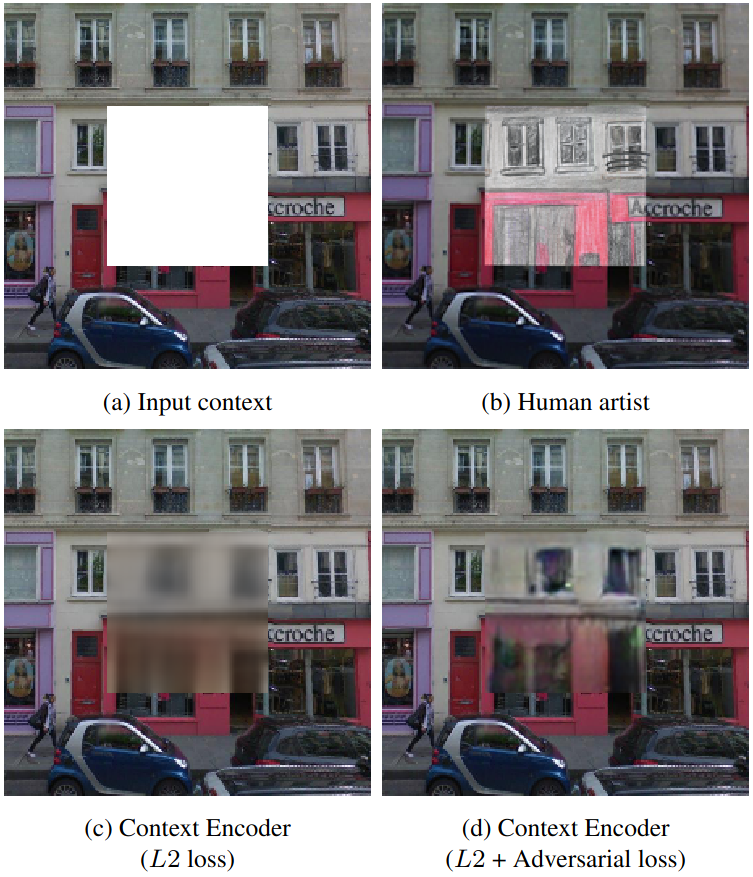
\includegraphics[width=0.7\linewidth]{figs/contextencodersLossComparison}
	\caption{مقایسه کیفی  استفاده از تابع هزینه نرم  ۲ در مقابل استفاده از یک تابع هزینه رقابتی در خروجی های تولید شده. 
		(a) عکس ورودی با یک قسمت از دست رفته 
		(b) یک انسان هنرمند مشکلی در ترمیم این تصویر ندارد 
		(c)
ترمیم خودکار تصویر با استفاده از \lr{Context Encoders} که توسط تابع هزینه بازسازی بر اساس نرم ۲ آموزش داده شده است.
	(d)
ترمیم خودکار تصویر با استفاده از \lr{Context Encoders} که توسط تابع هزینه رقابتی آموزش داده شده است.
}
	\label{fig:contextencoderslosscomparison}
\end{figure}



آن‌ها دریافتند  \lr{Context Encoders} بازنمایی ای یاد می‌گیرند که نه‌تنها ظاهر، بلکه معنای ساختارهای بصری را نیز در بر می‌گیرد. اثربخشی این ویژگی‌های یادگرفته‌شده به‌طور کمّی برای پیش‌آموزش شبکه‌های عصبی کانولوشنی (CNN) در وظایف طبقه‌بندی، تشخیص و قطعه‌بندی نشان داده شده است. علاوه بر این، \lr{Context Encoders} می‌توانند برای وظایف ترمیم معنایی تصاویر \lr{(Semantic Inpainting)} مورد استفاده قرار گیرند، چه به‌صورت مستقل و چه به‌عنوان نقطه شروع برای روش‌های غیرپارامتری.
\begin{figure}
	\centering
	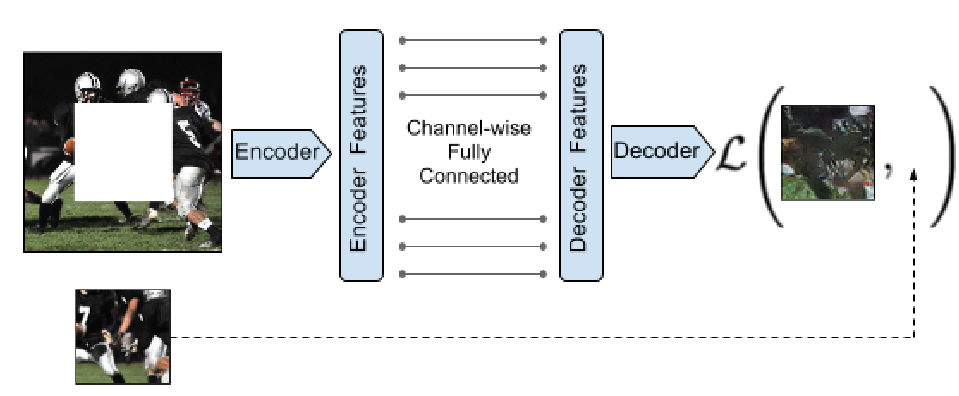
\includegraphics[width=0.7\linewidth]{figs/contextencodersArchitecture}
	\caption[معماری کلی Context Encoders]{
	تصویر زمینه از طریق بخش رمزگذار عبور داده می‌شود تا ویژگی‌هایی استخراج شوند که از طریق یک لایه کاملاً متصل کانال‌محور به رمزگشا متصل می‌شوند. سپس، رمزگشا نواحی حذف‌شده تصویر را تولید می‌کند.}
	\label{fig:contextencodersarchitecture}
\end{figure}

به دنبال این روش، روش های بسیاری بر پایه GAN ابداع شدند. 
\cite{caoLearningSketchTensor2021}
\cite{guoImageInpaintingConditional2024}
\cite{liRecurrentFeatureReasoning2020}
\cite{nazeriEdgeConnectGenerativeImage2019}
\cite{pengGeneratingDiverseStructure2021}

به عنوان مثال

این استراتژی‌ها همگی به دنبال این هستند که روش‌های مؤثری برای استخراج اطلاعات معتبر از نواحی شناخته‌شده تصویر به منظور پر کردن حفره‌ها پیدا کنند. هدف اصلی این رویکردها، بهره‌برداری بهینه از اطلاعات زمینه‌ای و استفاده از آن‌ها برای بازسازی نواحی گمشده است. با این حال، این روش‌ها هنوز با مشکلی اساسی روبرو هستند: از دست رفتن اطلاعاتی که در فرآیند نمونه‌برداری رو به پایین (\lr{Downsampling}) در شبکه‌های کانولوشنی رخ می‌دهد.  

این فرآیند نمونه‌برداری که برای کاهش ابعاد داده و افزایش بازده محاسباتی در شبکه‌های عصبی مورد استفاده قرار می‌گیرد، اغلب منجر به حذف جزئیات ظریف و اطلاعات ضروری می‌شود که می‌توانند برای بازسازی دقیق‌تر و واقعی‌تر مناطق گمشده نقش کلیدی ایفا کنند. بنابراین، یکی از چالش‌های مهم این است که چگونه می‌توان ضمن بهره‌گیری از مزایای نمونه‌برداری رو به پایین، تأثیرات منفی آن را کاهش داد و اطلاعات از دست رفته را تا حد ممکن حفظ کرد.